\section{Approach} \label{sec:Approach}

\subsection{Datasets}

Throughout our project, we apply a few datasets and analyze their generated
graphs. The datasets we use are, relatively speaking, orthogonal to each other -
They solve fundamentally different problems. As such, any similarities may be in
response to parameter changes, the network structure, or 'problem-solving'
itself.

Our first benchmark is the MNIST dataset \cite{MNIST Dataset}. This dataset
requires the tools of image recognition and classification, and is popular in
machine learning projects.

From there, we look at the Numenta Anomaly Benchmark dataset \cite{NAB Dataset}.
Anomaly detection is a problem that temporal neural networks generally
specialize in, so we analyze these as well.

Finally, we generate and analyze a network for the NFL Big Data Bowl dataset
\cite{NFL Dataset}. This network would perform prediction for the next 'play'
(e.g. pass or rush) based on the previous play's characteristics.

\subsection{Network Configuration}

Before discussing our network, we introduce our system. We define a temporal
liquid state machine (TLSM) as an input vector, encoded in time-based spikes,
followed by a reservoir of temporal neurons, and finally a singular output
column (with winner-takes-all lateral inhibition). The input vector uses
encoding strategies discussed in \cite{Encoding}, and the output column is
identical to the one described in \cite{TNN}.

\begin{figure}[h]
    \centering
    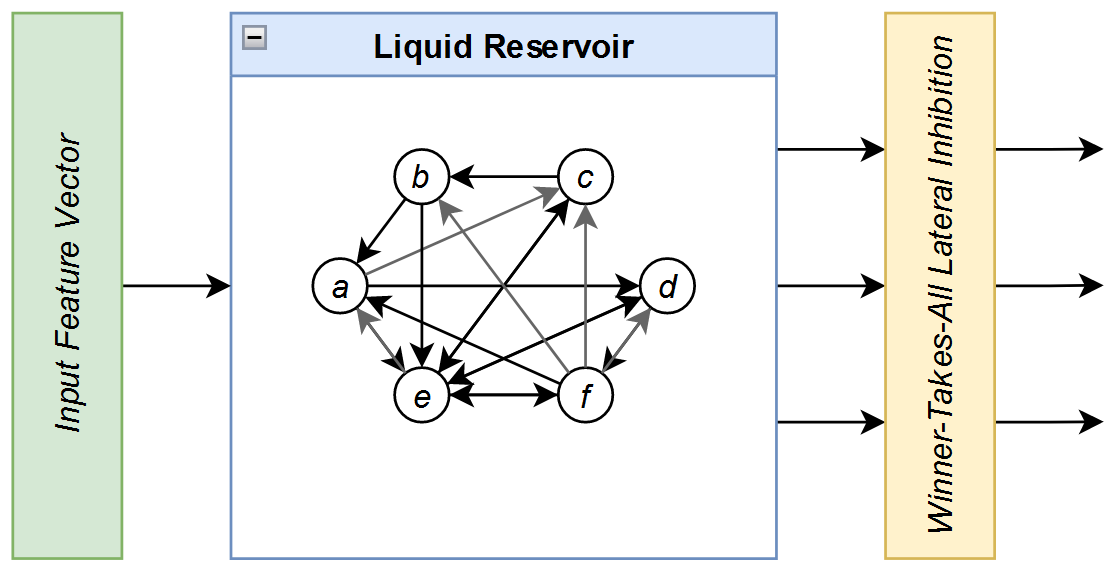
\includegraphics[scale=0.25]{tlsm_diagram.png}
    \caption{Diagram of a temporal liquid state machine (TLSM).}
    \label{fig:tlsm_diagram}
\end{figure}

The reservoir is the focus of network analysis, containing a series of neurons.
This graph of neurons will change over time with training and with STDP rules,
adding and removing connections arbitrarily in response to the inputs. The
neuron activation function is also a hyperparameter of the network.

Furthermore, a 'seed' configuration for the network may be specified, indicating
its initial connectivity. This seed configuration is generated through a
number of random graph algorithms, and is a hyperparameter of the network.

\subsection{Assumptions}

While we vary a variety of parameters (such as neuron activation function), we
assume that the underlying temporal neurons function as a strong analogue for
biological processes. This assumption allows us to generalize our results to
neural basis of cognition rather than design of artificial neural networks.

\subsection{Analysis}

The focus of analysis is the network generated within the liquid reservoir. This
liquid has nodes of neurons and edges of weighted synapses.

We test the robustness claim of \cite{LSM Constraints} by analyzing the
connectivity of these networks over their growth. We also analyze diameter in
order to understand the 'distance' between neurons in the network (and the
amount of time it takes for a spike to propagate).

\subsection{Research Questions}

Through these network features, and more, we aim to understand the following:

\begin{enumerate}
    \item Why did the network configure itself the way it did?
    \item How do networks of different problems compare to each other?
\end{enumerate}